\section{Heapsort}
HeapSort è un algoritmo di ordinamento che utilizza la struttura dati \emph{heap}.
Vedremo innanzitutto in cosa consiste uno heap, per poi trattare l'algoritmo e la sua 
complessità in termini di numero di confronti. Vedremo poi come uno heap possa
essere rappresentato nell'array stesso da ordinare, in modo tale da avere un implementazione in loco.

\subsection{La struttura dati \emph{Heap}}
Uno \emph{heap} è un \emph{albero binario quasi completo}, ovvero completo almeno
fino al penultimo livello, tale che la chiave contenuta in ogni suo nodo è maggiore 
o uguale alla chiave contenuta nei figli.\\
Poichè un albero binario di altezza $h$ contiene $2^{h+1} - 1$ nodi,
possiamo affermare che in uno heap di altezza $h$ il numero $n$ di nodi soddisfa $2^h \le n \le 2^{h + 1}$, da cui otteniamo
$h \le \log_2 n \le h + 1$ e dunque $h = \lfloor \log_2 n \rfloor$.\\
\begin{wrapfigure}{r}{7cm}
    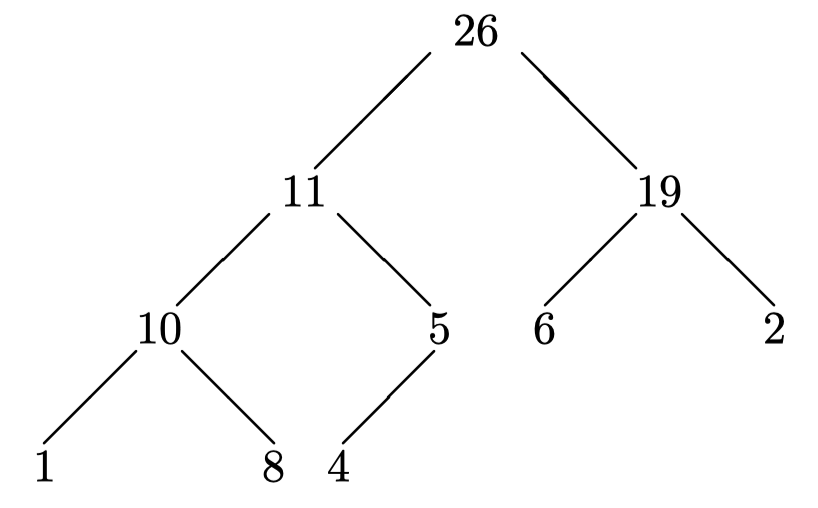
\includegraphics[scale = 0.5]{heap.png}
\end{wrapfigure}
La radice di uno heap contiene sempre la chiave maggiore. Pertanto, disponendo di 
uno heap contente le chiavi che dobbiamo ordinare, possiamo prelevare l'elemento che si trova
nella radice e collocarlo, come unico elemento, nella sequenza ordinata che dobbiamo
produrre come risultato, che costruiremo a partire dal fondo. Una volta fatto ciò possiamo
modificare la struttura in modo da riottenere uno heap ed applicare lo stesso procedimento.
\subsection{Sistemare uno heap}
Per risistemare uno heap applichiamo la seguente strategia.\\
Sostituiamo la chiave contenuta nella radice con quella contenuta nell'ultima
delle foglie, cioè quella che si trova più a destra nell'ultimo livello, rimuovendo
tale foglia. Tutti i nodi rispettano la condizione di heap, tranne la radice che potrebbe contenere 
una chiave inferiore rispetto a uno o entrambi i figli. In questo caso facciamo "scendere"
il dato presente nella radice, scambiandolo con quello di chiave maggiore tra i figli.
Se la condizione di heap non è rispettata dal figlio in cui abbiamo spostato il dato, 
iteriamo lo stesso procedimento su di esso.
\clearpage
\begin{figure}[h]
    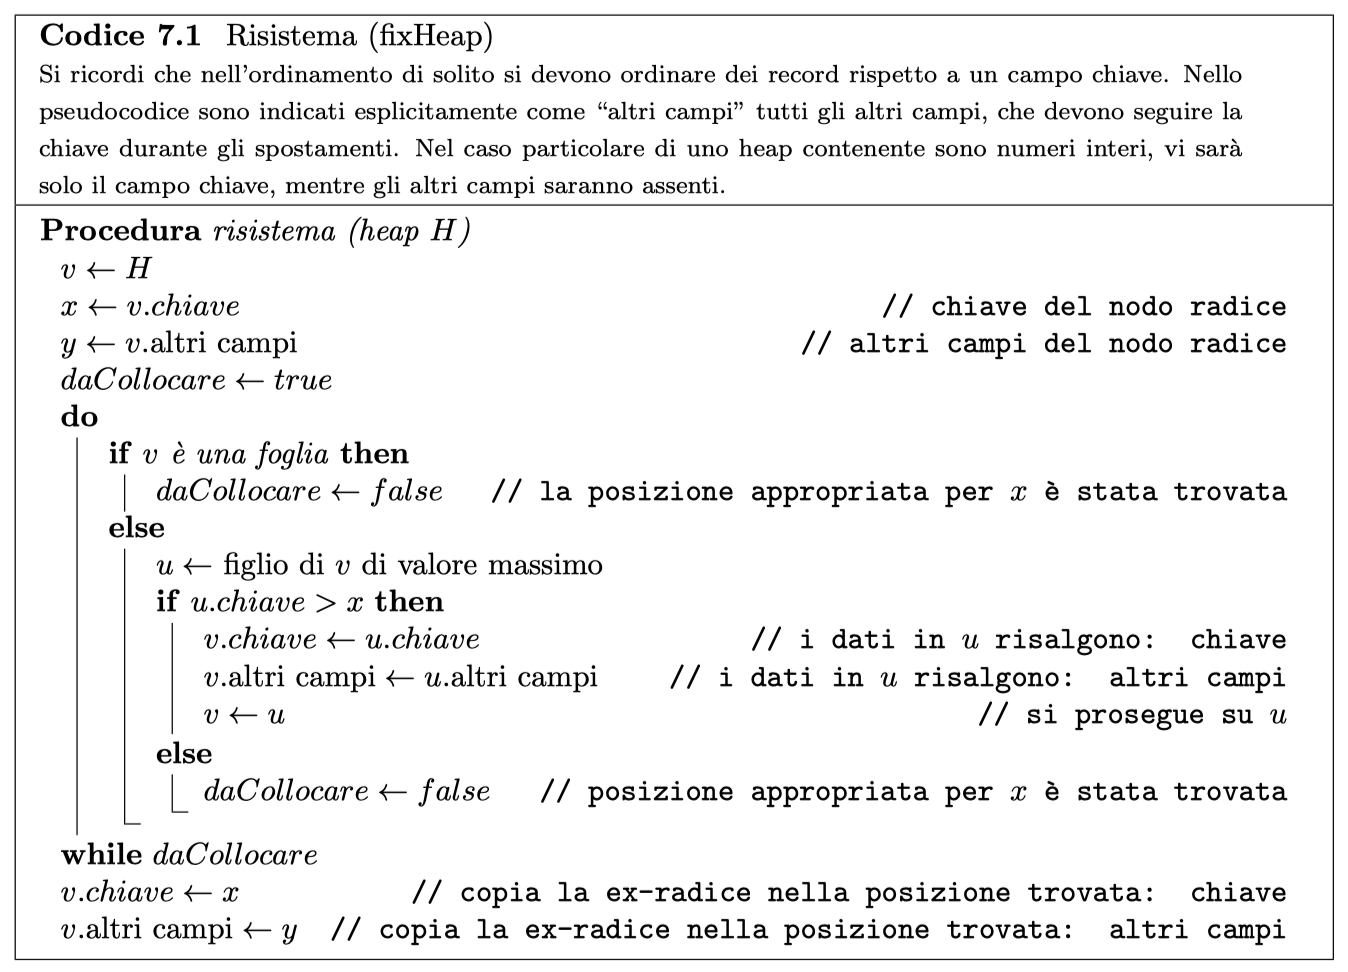
\includegraphics[width=\textwidth]{risistema.png}
\end{figure}
\subsubsection*{Numero di confronti}
Il numero di confronti usato da \texttt{risistema}, nel caso peggiore, $\Theta(h)$,
dove $h$ è l'altezza dello heap. Infatti il valore presente nella radice viene fatto scendere
lungo un cammino fino a raggiungere la posizione corretta che, nel caso peggiore,
potrebbe essere una foglia a distanza massima dalla radice. In questo processo, ad ogni passo viene
ispezionato un nodo lungo il cammino, determinando la chiave massima tra i figli e 
confrontandola con la chiave ispezionata. Pertanto per ogni nodo del cammino ho 2 confronti.
\clearpage

\subsection{Creazione di uno heap}
Supponiamo di disponere di un albero binario quasi completo le cui chiavi non rispettino però
la condizione di heap. Studieremo due soluzioni per trasformarlo in uno heap. La seconda soluzione è meno dispendiosa in 
termini di memoria.
\subsubsection*{Soluzione ricorsiva}
Strategia \emph{divide-et-impera}:
\begin{itemize}
    \item Se l'albero è vuoto non devo fare nulla
    \item Se l'albero non è vuoto trasformiamo ricorsivamente ciascuno dei due 
    sottoalberi sinistro e destro in heap; a questo punto tutti i nodi, eccetto la radice,
    soddisfano la condizione di heap. Applicando la procedura \texttt{risistema} possiamo trasformare l'albero in uno heap
\end{itemize}
\begin{figure}[h]
    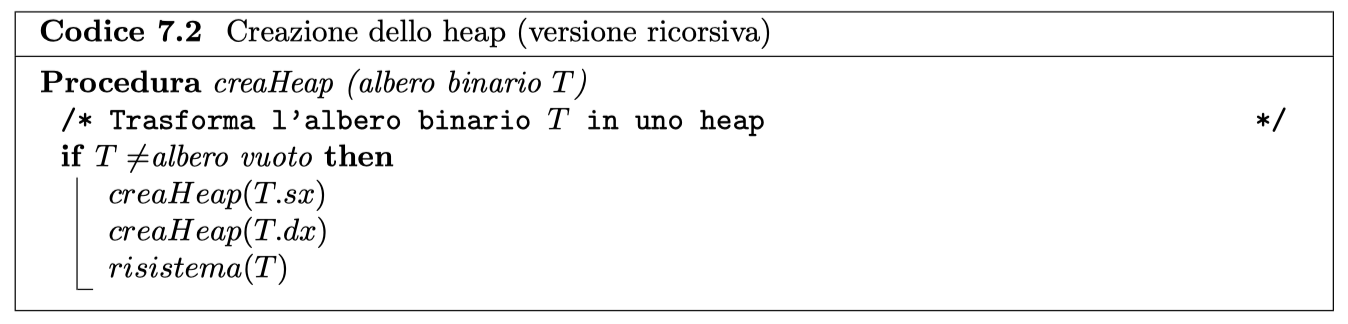
\includegraphics[width=\textwidth]{crea_heap_ricorsivo.png}
\end{figure}

\subsubsection*{Soluzione iterativa}
Anzichè costruire lo heap in maniera top-down, possiamo procedere in maniera bottom-up partendo
dalle foglie dell'albero. Ispezioniamo cioè l'albero a partire dall'ultima foglia, trasformando ogni sottoalbero
in uno heap. Quindi:
\begin{itemize}
    \item Iniziamo a considerare ciascun nodo di profondità $h$, da destra verso sinistra,
    e trasformiamo in heap il sottoalbero che ha tale nodo come radice (questi nodi sono foglie, quindi 
    i relativi sottoalberi sono già heap e per essi non occorre fare nulla).
    \item Passiamo a considerare ciascun nodo di profondità $h - 1$ (sempre da destra verso sinistra)
    e trasformiamo in heap il sottoalbero che ha radice in esso.
    \item Ripetiamo lo stesso procedimento considerando man mano profondità inferiori
    sino ad arrivare alla radice. A questo punto l'intero albero è uno heap.
\end{itemize}

\noindent Poichè i sottoalberi sono trasformati in heap a partire dal basso, quando in questo procedimento dobbiamo
trasformare in heap il sottoalbero $T_{x}$ che ha come radice un nodo $x$ di profondità $p$, i sottoalberi di $x$, avendo profondità
$p-1$, sono già stati trasformati in heap in passi precedenti. Dunque l'unico nodo di $T_{x}$ che potrebbe non
rispettare la condizione di heap è radice $x$. Quindi è sufficiente applicare \texttt{risistema}
per trasformare $T_{x}$ in uno heap.
\begin{figure}[h]
    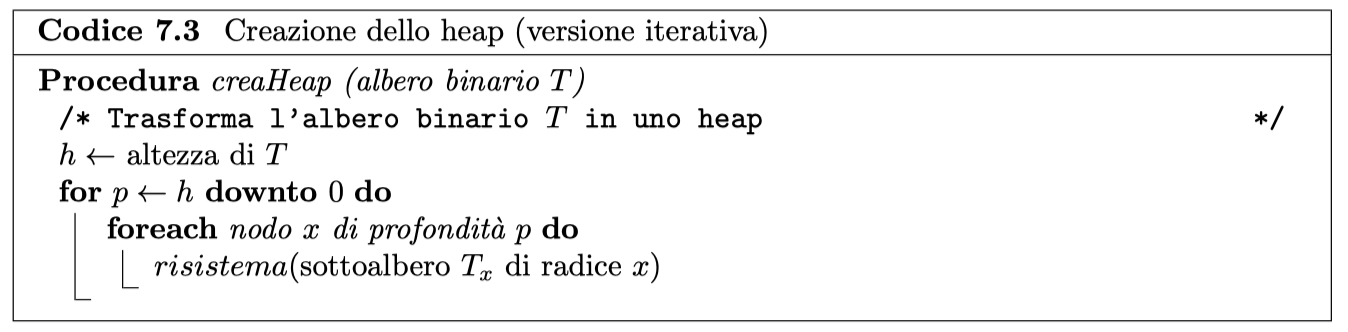
\includegraphics[width=\textwidth]{crea_heap_iterativo.png}
\end{figure}

\subsubsection*{Numero di confronti}
\texttt{creaHeap} chiama \texttt{risitema} un certo numero di volte, per sottoalberi di altezze differenti.
Il numero di confronti per trasformare in heap tutti i sottoalberi di profondità $p$ è 
$\Theta(h-p)2^p$. Nel ciclo esterno $p$ varia su tutte le profondità, cioè da 0 ad $h$.
Sommando su di esse otteniamo che il numero di confronti è $2^{h+1} - 2 - h$.\\
Essendo l'albero completo la sua altezza è logaritmica rispetto al numero di nodi. Questo 
permette di concludere che il numero di confronti di \texttt{creaHeap} è $\Theta(n)$, cioè lineare 
rispetto al numero di chiavi.

\subsection{Schema di \texttt{heapSort}}
\begin{figure}[h]
    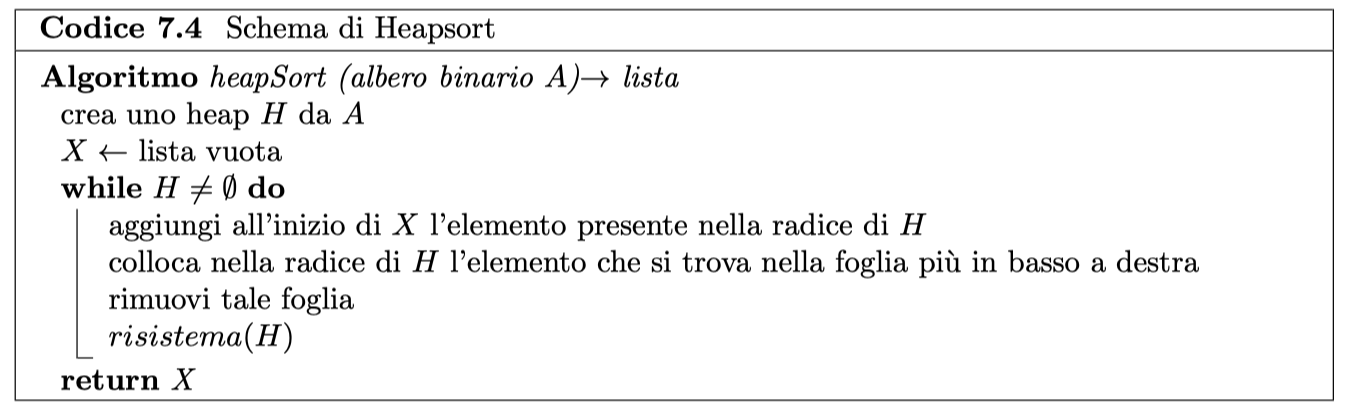
\includegraphics[width=\textwidth]{schema_heapsort.png}
\end{figure}

\subsubsection*{Numero di confronti}
\texttt{creaHeap} effettua $\Theta(n)$ confronti. Segue poi la parte iterativa in cui,
ad ogni passo, si preleva la radice e si risistema lo heap. Queste operazioni vengono ripetute
fino a svuotare lo heap, quindi $n$ volte. Risistemare lo heap utilizza, nel caso peggiore, un numero
di confronti proporzionale alla sua altezza, che è logaritmica. Dunque il numero
di confronti, nel caso peggiore, è $\Theta(n\log n)$.
\clearpage

\subsection{Ordinamento in loco di array tramite \texttt{heapSort}}
Si può implementare l'algoritmo in modo semplice senza ricorrere a strutture aggiuntive, servendosi
di una corrispondenza tra alberi binari quasi completi e array. Supponiamo di disporre del seguente array:

\begin{figure}[h]
    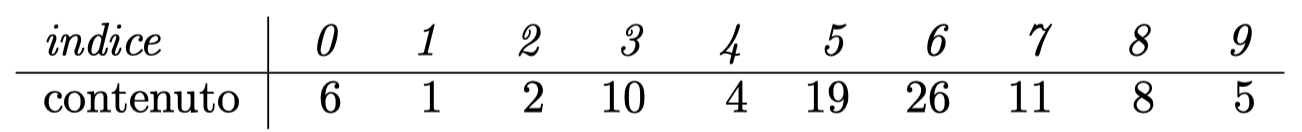
\includegraphics[width=10cm]{heap_array.png}
\end{figure}

\noindent Immaginiamo di collocare gli elementi dell'array nell'ordine in cui compaiono 
in un albero binario, riempiendo ciascun livello da sinistra verso destra a partire 
dalla radice, come in una visita in ampiezza. L'albero che otteniamo è il seguente:

\begin{figure}[h]
    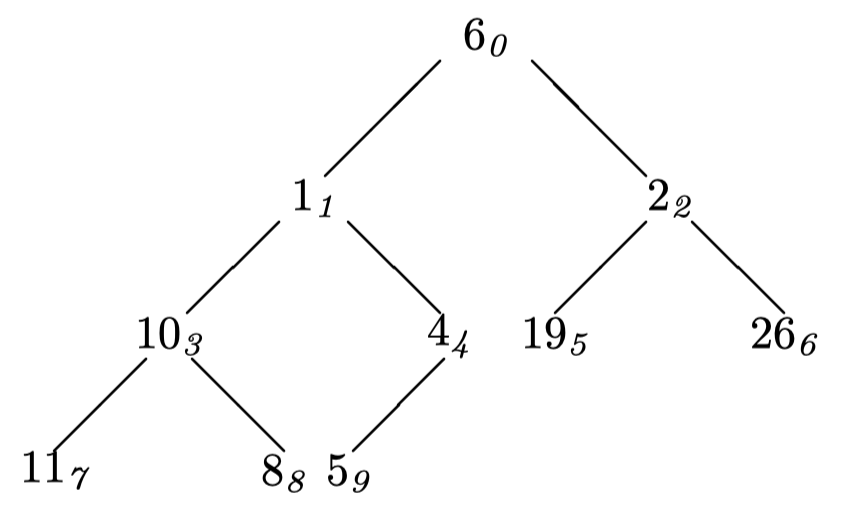
\includegraphics[width=7cm]{heap_albero_binario.png}
\end{figure}

L'albero è quasi completo, con le foglie dell'ultimo livello più a sinistra possibile.\\
Osserviamo che i figli del nodo che nell'array ha indice $i$ hanno, se esistono, indice
$2i + 1$ e $2i + 2$.\\
L'array che rappresenta un albero binario quasi completo è detto \emph{vettore posizionale}.\\
\begin{figure}[h]
    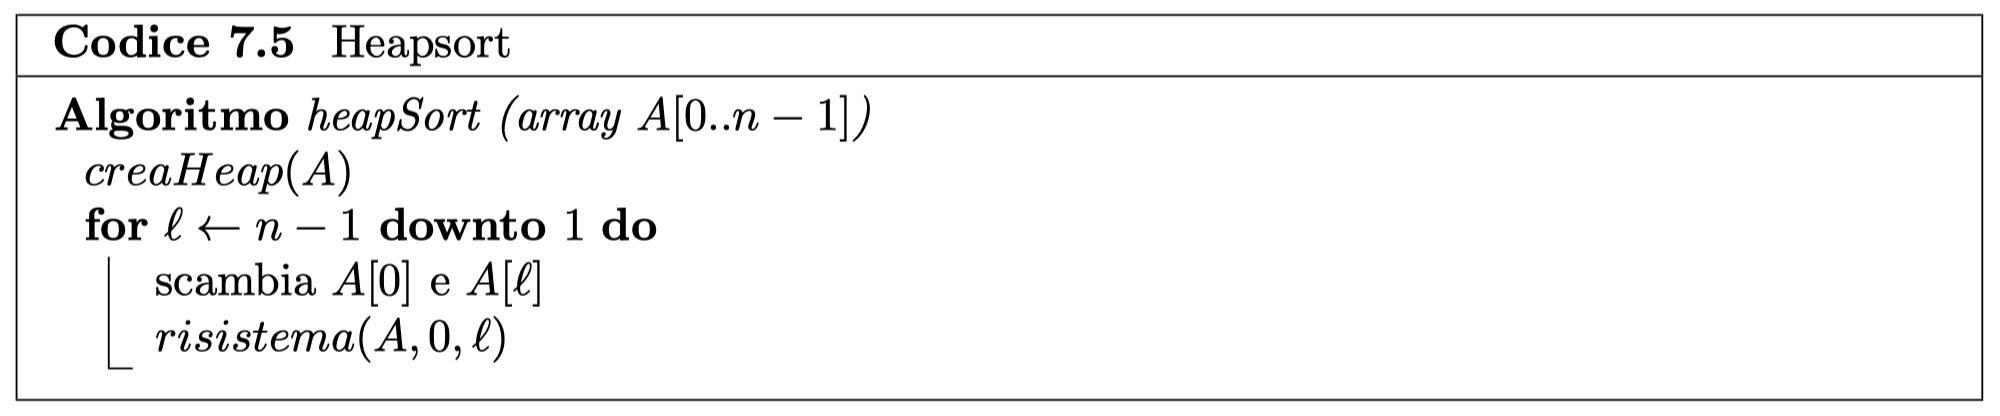
\includegraphics[width=\textwidth]{heapsort_array.png}
\end{figure}

Si possono modificare anche \texttt{creaHeap} e \texttt{risistema} affinchè lavorino
direttamente con l'array.

\begin{figure}[h]
    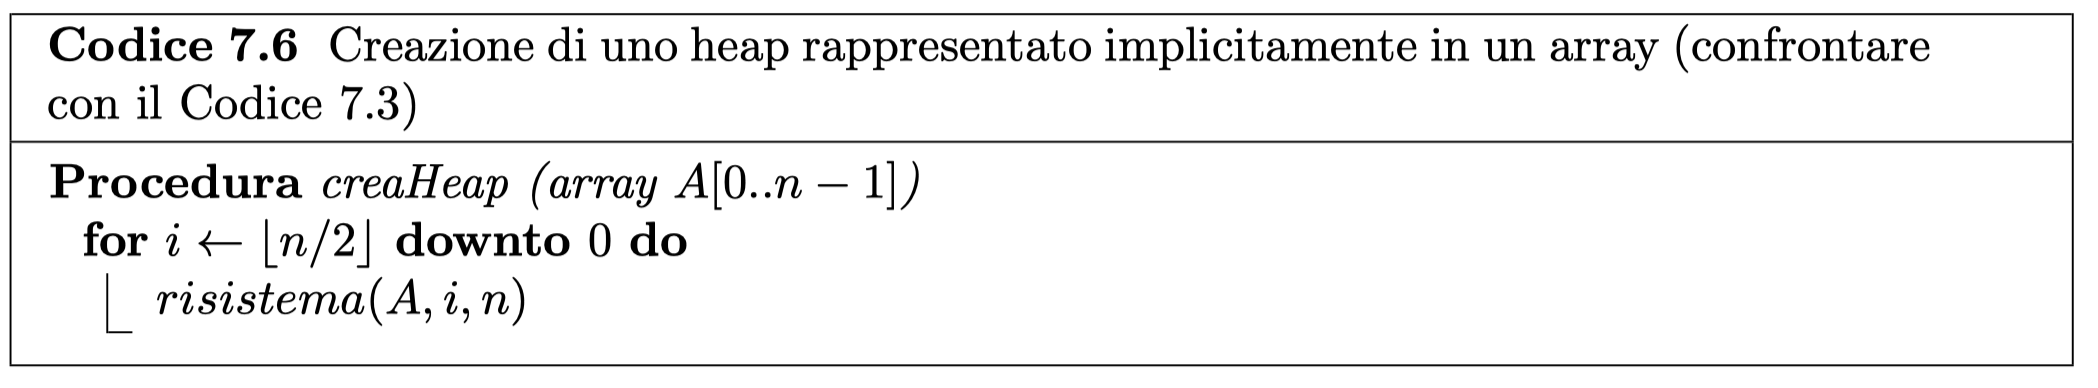
\includegraphics[width=\textwidth]{creaheap_array.png}
\end{figure}

\begin{figure}[h]
    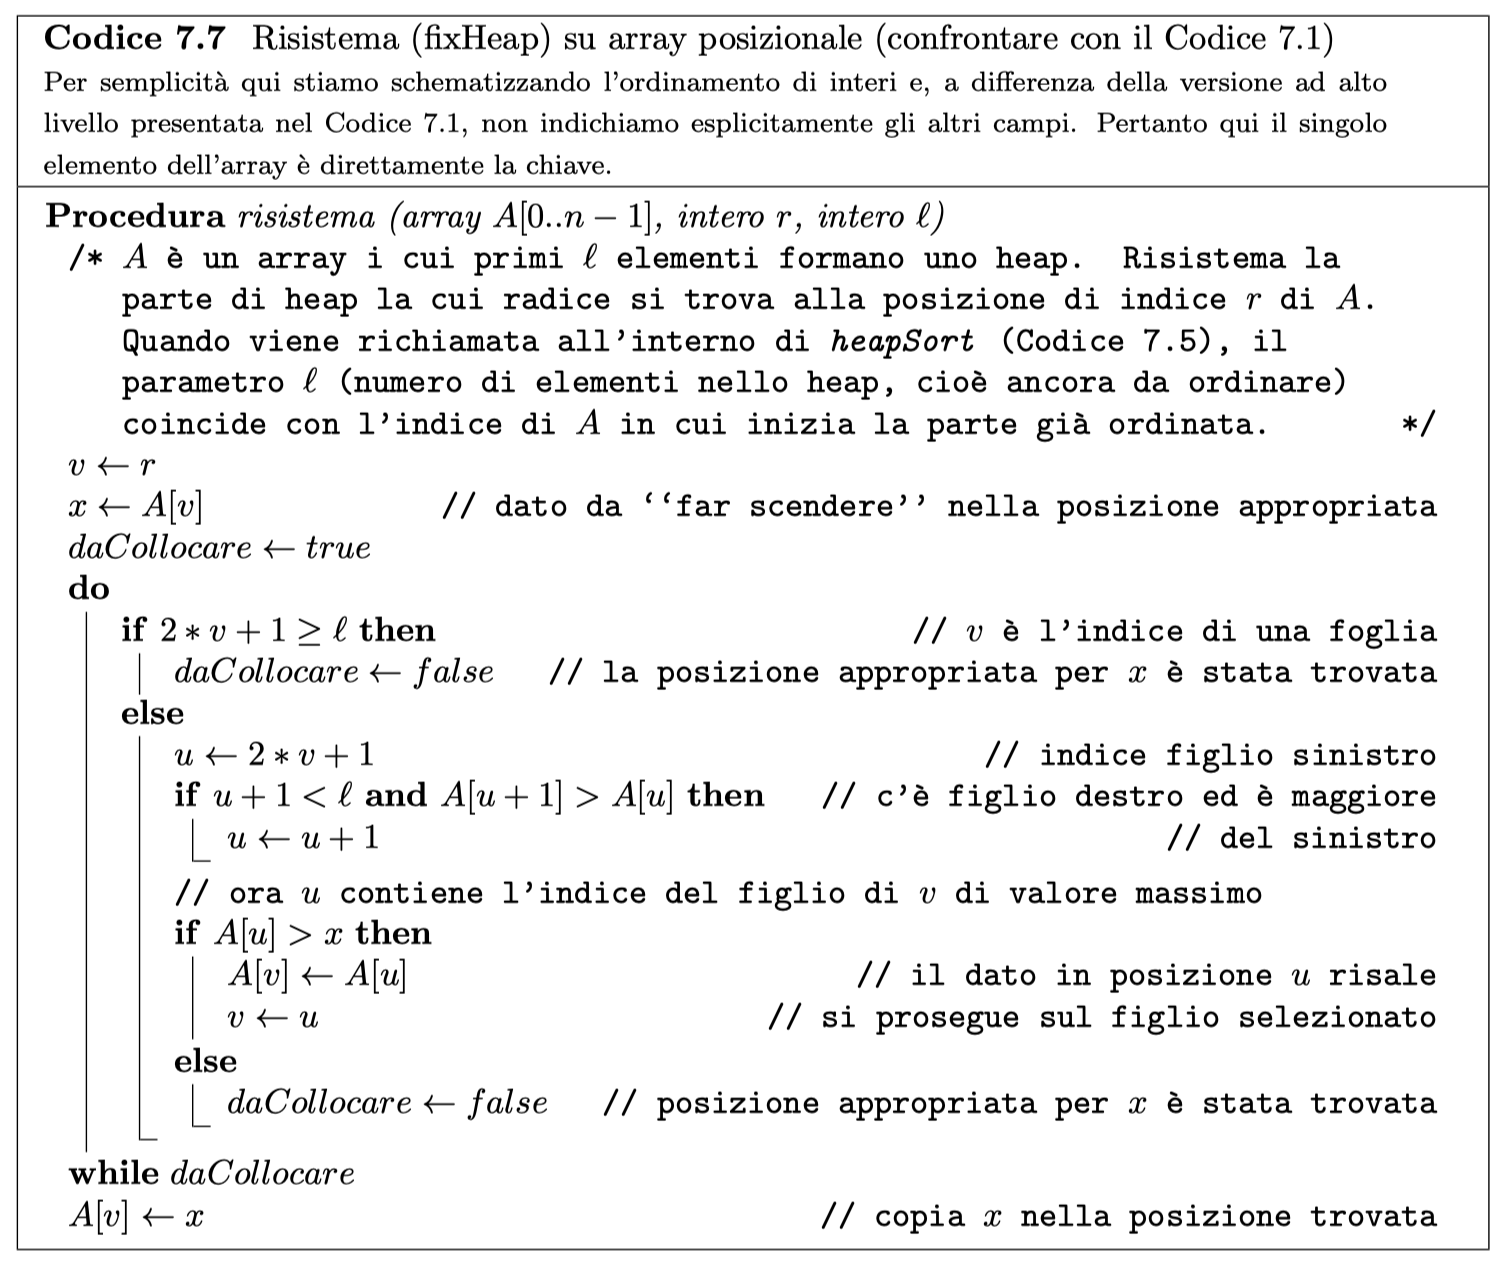
\includegraphics[width=\textwidth]{risistema_array.png}
\end{figure}
\clearpage

\subsection{Spazio}
Utilizzando la versione iterativa di \texttt{creaHeap} e l'implementazione in loco,
l'algoritmo utilizza spazio costante oltre all'array da ordinare.

\subsection{Costo operazioni su heap}
\begin{itemize}
    \item Trovare elemento di chiave massima $\rightarrow$ $O(1)$ passi
    \item Cancellare elemento di chiave massima $\rightarrow$ $\Theta(\log 1)$ passi
    \item Inserire un nuovo elemento $\rightarrow$ $\Theta(\log n)$ passi
    \item Cancellare elemento di chiave $x$ $\rightarrow$ $\Theta(\log n)$ passi
    \item Modificare la chiave di un elemento $\rightarrow$ $\Theta(\log n)$ passi
\end{itemize}

\subsection{Riassumendo}
\texttt{HeapSort} è un algoritmo di ordinamento in loco che, per ordinare $n$ elementi 
effettua $\Theta(n \log n)$ confronti. Pertanto, se ciascun confronto viene effettuato
in tempo $O(1)$, il tempo complessivo è $\Theta(n \log n)$.\\
Si può verificare che questo metodo non è stabile.
\clearpage